%-----------------------------------------------------------------------------------------------
%		\COMPdataPartManagement{} Design
%-----------------------------------------------------------------------------------------------

\section{\COMPdataPartManagement{} Design}
\label{sec:COMPdataBlockManagementDesign}

In this section, the design of the component \COMPdataPartManagement{} is described. Basic task of the component is to implement the actual generic parsing of data of a supported data format in a well-performing, yet flexible and extensible way.
% =======================================================================================================
\subsection{Basic Concept for Reading}%
\label{sec:BasicConceptforReading}%

In section \SectionLink{sec:RepresentingaDataFormat}, we discussed the approach that a data format is described in terms of a \emph{data format specification}, which basically is a description of how data is represented as a chunk of bytes in the data format. It breaks up such a chunk into different types of so-called data blocks that form a well-defined hierarchy (see \SectionLink{sec:TheContainerMetamodel}). Given such a specification and data block hierarchy, we define the following design decisions:

%%%% DD --> %%%%
\DD{dd:601}
{% Title
Data block instance classes defined in \COMPdataPartManagement{}
}
{% Short description
The instances for the different data block types are represented as Java classes in the \COMPdataPartManagement{} component which use the same names as in figure \ref{fig:II_GeneralModel}.
}
{% Rationale
As chunks of bytes are structured according to the metamodel and the data format specification describes them as such, it is quite clear the have to be instance of corresponding classes during parsing. These instances are also returned to the user and provide a clear, better-to-understand view on the data. Btw., having a metamodel but not transforming it into a class model seems to be quite nonsense.
}
{% Disadvantages
No disadvantages known.
}
%%%% <-- DD %%%%

%%%% DD --> %%%%
\DD{dd:602}
{% Title
Specification-driven Read Approach
}
{% Short description
Reading is heavily based on the description of the data format in its data format specification. The descriptions of lengths and types are used as basic assumption for parsing, especially magic keys for first identification.
}
{% Rationale
It is quite clear that otherwise, the data format specification would be quite useless and we would implement some data-format-specific and thus non-generic code again.
}
{% Disadvantages
Is it flexible enough? If we stick to a stiff specification, how to ensure that it is flexible enough for different data formats?
}
%%%% <-- DD %%%%

%%%% DD --> %%%%
\DD{dd:603}
{% Title
Reading and writing with \COMPmedia{}
}
{% Short description
Reading and writing is done using \COMPmedia{}, including use of its caching features.
}
{% Rationale
Again this is very clear.
}
{% Disadvantages
No disadvantages known.
}
%%%% <-- DD %%%%

Given these basic design decisions, we are ready to sketch a rough draft of how reading basically works. We first summarize the very fundamentals that we know this far:
\begin{itemize}
\item Data is represented as linear chunks of bytes whose structure is defined by the data format specification
\item The top-level data blocks for reading are containers
\item It is not clear which data format we have in front of us
\item A data block might get large, as we use long as data type (see \DesLink{dd:417})
\end{itemize}

Given the first two observations, we define the following:

%%%% DD --> %%%%
\DD{dd:604}
{% Title
Iterator approach for reading
}
{% Short description
  \LibName{} provides an iterator pattern for iterating top-level containers.
}
{% Rationale
As the basic structure of a chunk of data format bytes consists of linear disjoint containers and we need to do forward-reading, an iterator is a quite natural choice. Lists or other collection data types would be insufficient, because they would suggest that there is a finite number of containers. Iterators are a good fit for streaming, allowing virtually ``unlimited'' streams of containers.
}
{% Disadvantages
No disadvantages known.
}
%%%% <-- DD %%%%

Now we can define the basis approach of forward reading, i.e. what is done if we read a top-level container? Of course, first it is not clear which data format we have - identification is necessary, already introduced in \SectionLink{sec:MagicKeys}. Second, it might happen anytime that we hit end of medium, either expectedly or unexpectedly. The basic flow is defined in the following design decision and shown in figure \ref{fig:III_ForwardReading}.

\begin{figure}[htbp]
  \centering
  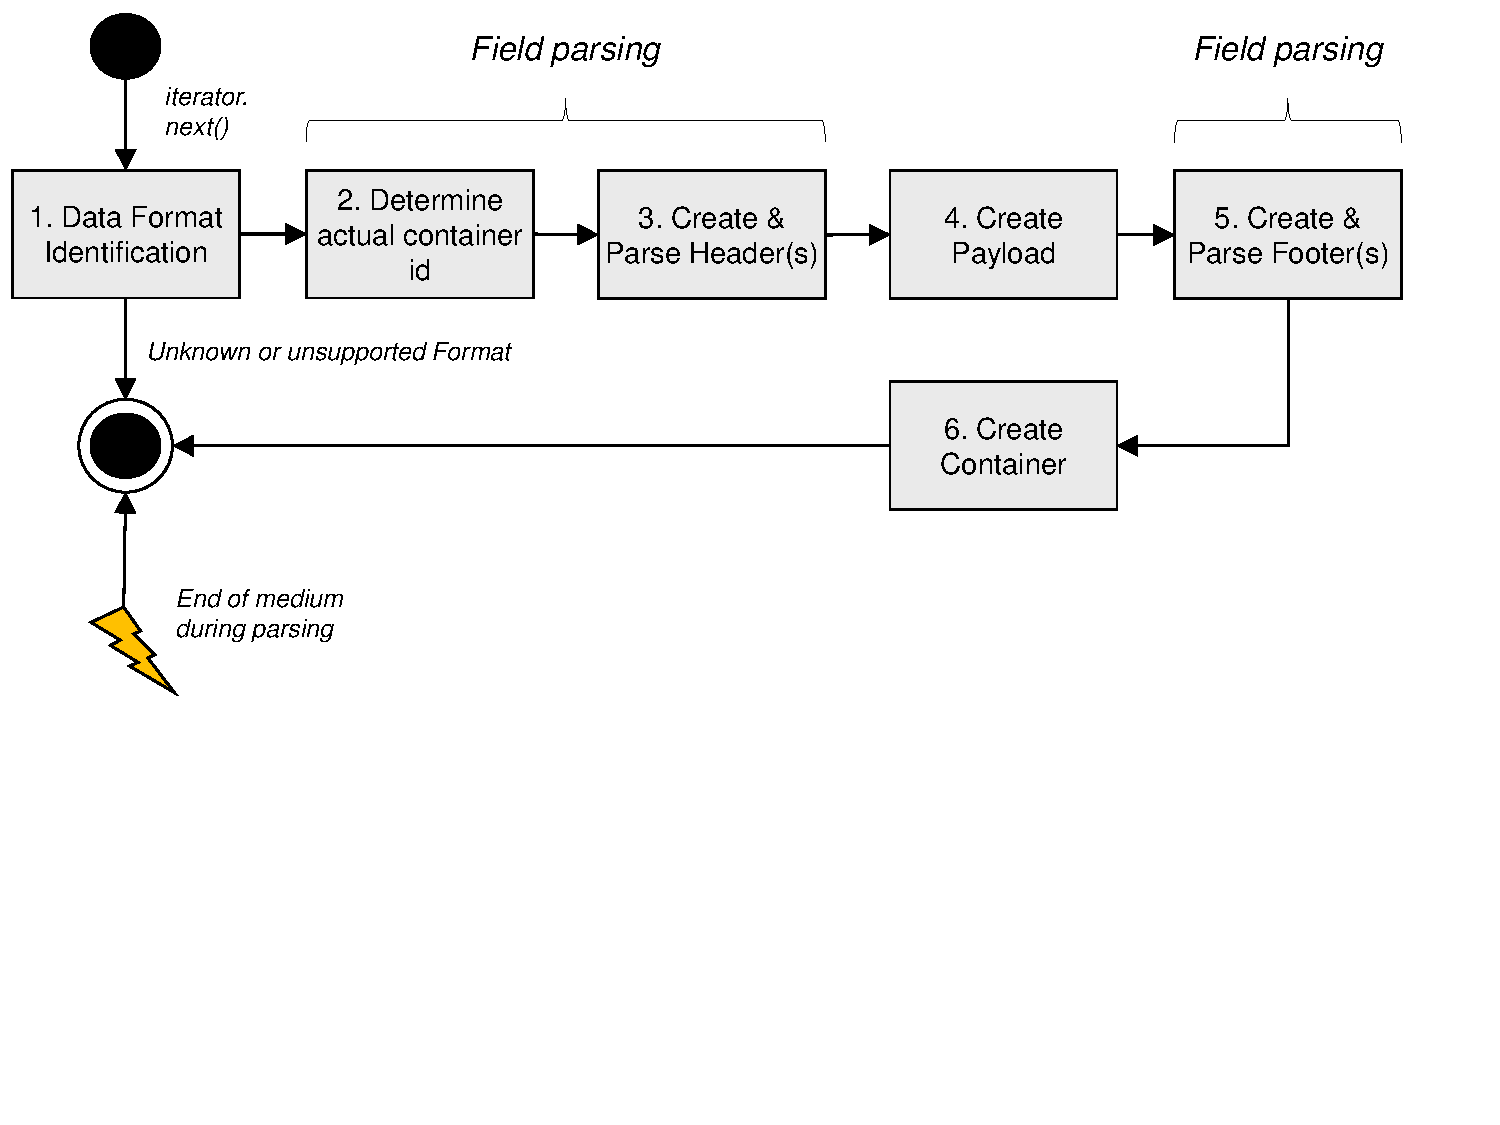
\includegraphics[width=1.0\linewidth]{figures/III_ForwardReading.pdf}
  \caption{Steps for reading data forward}
  \label{fig:III_ForwardReading}
\end{figure}

%%%% DD --> %%%%
\DD{dd:605}
{% Title
Steps of forward reading of top-level containers
}
{% Short description
  Forward reading of a single top-level container works as follows - whenever \texttt{next()} on the iterator is called to read the first or next container:
  \begin{enumerate}
  \item First, we do data format identification, i.e. finding out whether the data chunk ahead belongs to a data format the library supports - see \SectionLink{sec:MagicKeys} for details. If we cannot identify the data format, the process stops here with an exception.
  \item After identifying the data format, we need to identify which concrete container type and id we have, i.e. determining its structure and actual id at runtime; this is especially necessary for data formats supporting generic containers which is most of the container data formats out there, or multiple different container types. 
  \item Then, as we forward-read, the headers of the container are parsed, which means understanding their content. This includes determining if there are other headers or footers, and also the length of the container's payload.
  \item After heaving determined the payload length, the payload object itself is created. 
  \item Then, if there are any footers, they are at least created and ready to be parsed.
  \item Finally, the container is created which consists of the previously created headers, footers and payload
  \end{enumerate}
  It might happen that during this process, an expected or unexpected end of medium occurs. Expected it can only be during data format identification, in all other cases there seems to be a corruption in the data or parallel changes, as the parsing metadata indicates a size which is not matching reality.

  During steps 2, 3 and 5, fields need to be parsed which is a special discipline discussed later.
}
{% Rationale
The process is aligned at the structure of a container and typical for forward reading.
}
{% Disadvantages
No disadvantages known.
}
%%%% <-- DD %%%%

Btw:
%%%% DD --> %%%%
\DD{dd:605a}
{% Title
Steps of forward reading for nested containers
}
{% Short description
These are nearly identical except that data format identification is unnecessary.
}
{% Rationale
Nested containers are other than the fact that the data format is already known in no way different to top-level containers.
}
{% Disadvantes
No disadvantages known
}
%%%% <-- DD %%%%

% =======================================================================================================
\subsection{Buffering, Caching and Lazy Reading}%
\label{sec:ReadingSteps}%

\COMPdataPartManagement{} uses the features of \COMPmedia{} for caching as described in \SectionLink{sec:PerfMedia}. These features are also used for buffering, i.e.
%%%% DD --> %%%%
\DD{dd:606}
{% Title
General buffering using maximum read-write block size is done - for each overlap buffer the next block
}
{% Short description
  Most of the read operations in \COMPdataPartManagement{} do a buffering before accessing data. They always buffer at most maximum read-write block size of bytes. If a buffering call detects that the start offset of buffering plus maximum read-write block size exceeds current buffered data, it buffers the next block starting behind the currently buffered data with at most maximum read-write block size of bytes.

  This decision strongly bases on the critical design decision \DesLink{dd:438a} for a sensible handling of objects (e.g. fields) overlapping two consecutive byte blocks read.
}
{% Rationale
Reading byte by byte or field by field would be nonsense from performance point of view. The maximum read-write block size is a natural fit for buffering. The approach of buffering the next block when an overlap is detected is sensible as it leads to less cache fragmentation. The previously cached consecutive block will not fall out of the cache thanks to design decision \DesLink{dd:438a}.
}
{% Disadvantages
No disadvantages known.
}
%%%% <-- DD %%%%

Now the question arises: Where to buffer exactly to ensure that there is no ``buffer gap''?

%%%% DD --> %%%%
\DD{dd:606a}
{% Title
Buffering at start of container and field reading
}
{% Short description
  It turned out to be fully sufficient if we do the following:
  \begin{itemize}
  \item Buffer at start of container identification/reading: Whenever it is checked if a container with a given type and id during container identification phase is done, we first buffer read-write block size of bytes. As this size has a lower bound (see \DesLink{dd:438a}) with a sensible default, this way all usual headers are already buffered, leading to speeding up data format identification for top-level containers.
  \item Buffer at start of field reading: Whenever a single field of a header, footer or payload is read, buffering is done. Due to \DesLink{dd:606}, any overlapping bufferings will actually read the next block in addition, ensuring that always as sensible amount of future bytes is pre-buffered. This case also covers field based payload.
  \end{itemize}
}
{% Rationale
Thus, even if we have unusually long headers, footers or field-based payload, there is never a buffering gap.
}
{% Disadvantes
No disadvantages known
}
%%%% <-- DD %%%%

A very basic mechanism of container data formats is that they allow seeking and skipping based on containers, that means the decoders might just need to check a container header to find out if they are interested in the data it contains, and if not simply go on reading with the follow-up container. For this, most if not all data formats specify the size of the container in its header or footer. To fully support this, we define some kind of lazyness as follows:

%%%% DD --> %%%%
\DD{dd:607}
{% Title
Lazy payload
}
{% Short description
Any field-based or container-based payload is lazy by default, i.e. its bytes are first read only when explicitly requested by the user. A sole exception is in place for stream-based media (see upcoming design decision). 
}
{% Rationale
This way, we do not read unnecessary data the user might never look at, especially allowing to skip over large containers without risking out of memory and long read times, just perfectly meeting requirement \SectionLink{sec:REQ009LesenSchreibenGrosse}.
}
{% Disadvantes
No disadvantages known
}
%%%% <-- DD %%%%

As streams are non-random-access media, the question arises what we do with the bytes of a stream. It is no good idea to skip the payload byte here - what if the user wants to closely look at them? There is no other choice than to still cache them. The same is true for rather ``exotic'' formats such as Lyrics3v2 where the payload size is not contained in a header, but only in the footer.

%%%% DD --> %%%%
\DD{dd:608}
{% Title
Fully cache payload for stream-based media and formats without size field
}
{% Short description
  For stream-based media, the whole payload data must be fully read to at least have a chance that the user can look at it later. It might happen that the maximum cache size is exceeded in which case the first bytes of the payload might fall out of the cache.

For formats not having a static payload size and not having a size indicator in its header, the payload must be fully read in entirety to know its size. This also leads to potentially filling up the cache. 
}
{% Rationale
  There is no other way for streams than grabbing the bytes when looking at them - streams are just one time read.

  For the special case of formats not having a payload size in their header, see \DesLink{dd:529d}.
}
{% Disadvantes
No disadvantages known
}
%%%% <-- DD %%%%

% =======================================================================================================
\subsection{Container Context Information}%
\label{sec:ContainerContextInformation}%

In section \SectionLink{sec:FieldFunctions}, we already mentioned the \emph{parsing metadata} that is vital for understanding and reading a container. This information is tagged as such by each extension in the form of field functions that link fields to target blocks they refer to. This information is of course relevant for generically parsing a container at runtime. As soon as you encounter e.g. a field that contains the size of the container's payload during parsing, you have to store this size somewhere to be accessible later when actually parsing the payload.

Here, we summarize all the parsing metadata known at one point in time during container parsing as the \emph{container context information}. However, the container context information shall not only be a simple map storing the already known field functions, but it is intended to be more:

%%%% DD --> %%%%
\DD{dd:620}
{% Title
\texttt{ContainerContext} provides sizes, counts, byte orders and character encoding of all data blocks in a container; it is available in each data block; one instance per container
}
{% Short description
A helper class \texttt{ContainerContext} provides sizes, counts, byte orders and character encoding of \emph{all} data blocks in the current container. That means it not only stores the field functions refering to some of them, but also knows about static sizes, static occurrences, default byte orders and character encodings etc. It is an attribute of each data block such that it can be accessed from most places during as well as after parsing. The details of size determination are described in \SectionLink{sec:SizeDetermination}, the details of count determination in \SectionLink{sec:CountDetermination}.
}
{% Rationale
Having just one place that not only stores field function values but also knows in a more abstract way how to determine sizes, counts, byte orders and character encodings allows for better separation of concerns. This also allows to pass around corresponding objects to everywhere you need this information in contrast to having this logic only in a reader class that is not availabe anywhere else after parsing.
}
{% Disadvantes
No disadvantages known
}
%%%% <-- DD %%%%

One question that comes up here: How about parsing metadata available in the top-level container, but needed in a child container? We define:

%%%% DD --> %%%%
\DD{dd:621}
{% Title
\texttt{ContainerContext} contains a reference to the direct parent container's context and searches the parent for metadata if none is found in itself
}
{% Short description
\texttt{ContainerContext} contains a reference to the direct parent container's context (if any). If it cannot come up with a size, count, byte order or character encoding itself, it asks the parent for such metadata.
}
{% Rationale
This way, parsing metadata only defined in the top-level container headers can be transported to children deeper in the hierarchy.
}
{% Disadvantes
No disadvantages known
}
%%%% <-- DD %%%%

% -------------------------------------------------------------------------------------------------------
\subsubsection{Size Determination}%
\label{sec:SizeDetermination}%

How to determine the sizes of data blocks before parsing? It is clearly necessary to know the size of a container in advance to be able to parse or skip it. Unfortunately, all data formats seem to follow a distinct strategy of how to specify sizes as indicated around design decision \DesLink{dd:540}.

The cases we have to handle are summarized as follows:
%%%% DD --> %%%%
\DD{dd:640}
{% Title
Cases for size determination
}
{% Short description
  The easiest \textbf{Case 1:} Static size indicated in the specification. If a data block's specification indicates a static size, this size is taken during parsing.

  Otherwise, the data block has a dynamic size which breaks down to the following cases:
  \begin{enumerate}
  \item[\textbf{Case 2:}] The data block's size is directly indicated by another field that must be parsed before (usually in header or footer) - Note that this size might include the size of other blocks in addition, see \DesLink{dd:542} and the discussion around for more details. Here, ``directly'' means that the field is a numeric value greater or equal to the size, and we do not need to calculate something.
  \item[\textbf{Case 3:}] The data block's size is indirectly indicated by other fields that must be parsed before (usually in header or footer). ``Indirectly'' means that the field is not just single or summed size contained in a field, but there is a more complex calculation of combining multiple field values to calculate the size. This is e.g. the case for the size of the MP3 container payload or the Ogg page payload and packet part sizes.
  \item[\textbf{Case 4:}] The data block is payload consisting of fields or containers, and there is no size indicator at all. However, it is clear how to determine the sizes of all children of the payload block, and thus the size of it is the sum of the sizes of all its children. This is e.g. the case for Lyrics3v2 tag payload.  
  \item[\textbf{Case 5:}] The data block is a terminated field, i.e. its size must be determined by finding its termination. The handling of this case is defined in \SectionLink{sec:TerminatedFields}.
  \item[\textbf{Case 6:}] None of the other cases applies, but at least the overall remaining size of the parent data block is known. Take the remaining size of the parent data block as size of the data block.
  \end{enumerate}

  \LibName{} supports exactly those cases. Despite case 5, they are implemented in the \texttt{ContainerContext}, see \SectionLink{sec:ContainerContextInformation}.
}
{% Rationale
The cases come from analyzing different data formats \LibName{} is required to support, so it is sufficient to consider only those (if any others exist). Why is case 5 not implemented in \texttt{ContainerContext}? The reason is that finding termination bytes requires parsing itself, so it must be implemented in the reader.
}
{% Disadvantes
No disadvantages known
}
%%%% <-- DD %%%%

Case 1 is already clear how to deal with, case 5 is treated later in \SectionLink{sec:TerminatedFields}. Thus we are left to deal with cases 2 to 4. First of all, we consider case 3:

%%%% DD --> %%%%
\DD{dd:641}
{% Title
Complex size calculation from fields done in custom implementation via \texttt{SizeProvider}
}
{% Short description
Data format extensions are allowed to register a custom \texttt{SizeProvider} implementation which calculates the size of a data block as required by the format. This is used for Ogg, ID3v2.3 extended header size and MP3.
}
{% Rationale
More flexibility also for yet other future formats.
}
{% Disadvantes
No disadvantages known
}
%%%% <-- DD %%%%

Case 4 is handled as follows:
%%%% DD --> %%%%
\DD{dd:642}
{% Title
Determine payload size by reading all children
}
{% Short description
In case 4 of \DesLink{dd:640}, the size of the payload is calculated by reading all children, may it be containers or fields, and summing up their sizes. If at least one of their sizes could not be determined, this is a runtime exception.
}
{% Rationale
Straightforward and not too complex in terms of ``lazyness''. If the data formats design is fucked up, the implementation cannot easily work around it.
}
{% Disadvantes
No disadvantages known
}
%%%% <-- DD %%%%

Now we have case 2 left. This one is adressed with using field functions - potentially referring to multiple consecutive blocks as indicated by \DesLink{dd:540}. We clarify how it works by summing up the whole progress of size determination in total:

%%%% DD --> %%%%
\DD{dd:644}
{% Title
Size determination process
}
{% Short description
  Whenever the size of a single data block needs to be determined, the following steps are performed in the given order of precedence:
\begin{enumerate}
\item (Outside of \texttt{ContainerContext}) If the data block is a terminated field without fixed size, search for the termination character (case 5)
\item Otherwise if the current data format has a registered \texttt{SizeProvider} (see \DesLink{dd:641}), first ask this instance if it can provide a defined size (includes also case 3)
\item Otherwise if the data block has a static size according to its specification, take this size (case 1)
\item Otherwise if the current \texttt{ContainerContext} has a \texttt{SizeOf} field function, take the size indicated by the \texttt{SizeOf} field (part 1 of case 2)
\item Otherwise if the current \texttt{ContainerContext} has a \texttt{SummedSizeOf} field function for multiple data blocks and the sizes of all other blocks are known, take the \texttt{SummedSizeOf} field's value minus the summed size of the other data blocks (part 2 of case 2) - How to avoid an infinite loop here? This has been treated in design decision \DesLink{dd:541} and is also discussed with an example after this design decision.
\item Otherwise if the data block is a concrete data block that is derived from a generic data block, it is checked if there is a known size for the generic id  
\item Otherwise if the parent \texttt{ContainerContext} has a \texttt{SizeOf} field for it, take the size of the parent \texttt{ContainerContext}
\item Otherwise if the data block is a field or payload and the remaining parent size is known, take the remaining direct parent size as its size (case 6)
\item (Outside of \texttt{ContainerContext}) Otherwise if the data block is a payload block, read all its children and sum up their sizes (case 4)
\end{enumerate}
}
{% Rationale
The order of steps clearly focusses on least complexity first and tries to avoid unnecessary lookups by first considering fixed sizes and custom size providers.
}
{% Disadvantes
No disadvantages known
}
%%%% <-- DD %%%%

Some subtle point in determining sizes of single data blocks whose \texttt{SummedSizeOf} field is the sum of multiple consecutive data blocks is: If we want to determine the size of a single one, we have to determine the size of all the others, sum this size and subtract it from the value stored in the \texttt{SummedSizeOf} field. If for some stupid reason there are multiple data blocks included with a dynamic size, this could end up in an infinite loop such as for ID3v2.3: Size of payload needs to be determined, thus determine the size of the extended header first. However, the size of the extended header is also dynamic. The implementation would see that it would need the size of the payload to calculate the size of the extended header and thus call the first function again... To avoid this crap, we already stated the validity criteria in \DesLink{dd:541}.

% -------------------------------------------------------------------------------------------------------
\subsubsection{Count Determination}%
\label{sec:CountDetermination}%

Here we discuss how the determination of the number of occurrences of a data block (i.e. count determination) works. First of all, we can state that the number of payload containers is always 1, so no need to consider this case. For all other types of data blocks, there can be 0 to multiple occurrences.

The process to handle is summarized as follows:

%%%% DD --> %%%%
\DD{dd:645}
{% Title
Count determination process
}
{% Short description
  Whenever the count of a single data block needs to be determined, the following steps are performed in the given order of precedence:
\begin{enumerate}
\item If the current data format has a registered \texttt{CountProvider}, first ask this instance if it can provide a defined size
\item Otherwise if the data block has a static number of occurrences according to its specification, take this count
\item Otherwise if the data block is optional, i.e. either is present once or not at all, and if the current \texttt{ContainerContext} has a \texttt{PresenceOf} field function, take 1 as count if its presence is indicated by the flags, 0 otherwise
\item Otherwise if the current \texttt{ContainerContext} has a \texttt{CountOf} field function, take the count indicated by the \texttt{CountOf} field
\item Otherwise if the parent \texttt{ContainerContext} has a \texttt{CountOf} field for it, take the size of the parent \texttt{ContainerContext}
\end{enumerate}
}
{% Rationale
The order of steps clearly focusses on least complexity first and tries to avoid unnecessary lookups by first considering fixed counts and custom count providers.
}
{% Disadvantes
No disadvantages known
}
%%%% <-- DD %%%%

% =======================================================================================================
\subsection{Field Parsing}%
\label{sec:FieldParsing}%

Field parsing is the most complex part of reading data format bytes. It requires answers to following questions:
\begin{itemize}
\item How to determine the size of the field? - This has been answered already in \SectionLink{sec:SizeDetermination}, except the case of terminated fields which we treat here
\item How to determine the number of occurrences of a field, especially the case of optional fields? - This has been answered already in \SectionLink{sec:CountDetermination}
\item Which byte order (for numeric fields) and character encoding (for string or enumerated fields) needs to be used when? - This has been answered already in \SectionLink{sec:ContainerContextInformation}
\item How to convert the binary field value to an interpreted one?
\item How to use caching during field parsing?
\end{itemize}

% -------------------------------------------------------------------------------------------------------
\subsubsection{Terminated Fields}%
\label{sec:TerminatedFields}%

Terminated fields are those fields with a dynamic length that is not given by the value of another field, but these fields are delimited by a sequence of termination bytes or characters. 

Terminated fields are worst-case for parsing: First of all you never know when it ends, and second you have to deal with strings which brings different encodings into play.

Let's deal with the first problem, the unknown length. Of course, in the ``usual'' case a terminated field is still a field and thus relatively small. We will only rarely encounter terminated fields longer than several KB. In order to be fully generic, one needs to deal with the worst case of fields having up to \texttt{Long.MAX\_VALUE-1} as size. Having said this, also block-wise reading is required as we do not want to risk out-of-memory conditions by soaking too much bytes into memory. One could come up with the idea of using some upper bounds for reading data, i.e.:
\begin{itemize}
\item \textbf{Case 1:} The current total medium size as well as the exact size of a parent of the field is known - E.g. for ID3v23 text frames, the frame size and thus payload size is known, but there is a terminated text payload field; for file and byte array media, the medium length is also known.
\item \textbf{Case 2:} The current total medium size is unknown, yet the exact size of a parent of the field is known - Take an ID3v23 text frame on an input stream medium as an example.
\item \textbf{Case 3:} The current total medium size is known, but the exact size of a parent of the field is unknown - Take an APEv2 item header on a file or byte array medium as an example. Here, the item key is terminated, and the size of the parent header is unknown as it is only determined by the sum of the field sizes and not - in addition - by any size indicators.
\item \textbf{Case 4:} Neither current total medium size nor the exact size of a parent of the field is known - So APEv2 item header on an input stream medium is an example.
\end{itemize}

%%%% DD --> %%%%
\DD{dd:650a}
{% Title
Block-wise reading for finding field termination
}
{% Short description
Block-wise reading is necessary in order to find field termination. According to \DesLink{dd:438}, we do not read more than the configured maximum read-write block size in bytes from the medium at once. Actually, we \emph{always} read the configured maximum read-write block size and do not take into consideration any additionally known upper bounds such as the remaining parent byte count or remaining medium length (if available). If an end of medium is encountered during reading a block of data, we scan for the termination within the actually read bytes. Otherwise the next block is read for scanning for termination bytes and so on. However, we can at least take into account any available bounds for finding out if we need to search further or we can skip the process: If the already read byte count is bigger than the remaining parent byte count, we should skip as a data corruption might be present.
}
{% Rationale
Block-wise reading avoids out-of-memory conditions and is a compromise between reading too much and reading too few bytes at once. Of course this compromise comes with the cost of added complexity. We mitigate this complexity by not coming up with further ``optimizations'' such as only reading up to a known upper bound like the medium end or parent end. In the end, both might not be known, especially in case 4, thus anyway we have to do a ``blind'' reading in this case.
}
{% Disadvantes
Added complexity, but in conformance with \DesLink{dd:438}. The complexity is adressed as specified in the rationale.
}
%%%% <-- DD %%%%

Regarding strings and their encoding: First of all, we remember that only string and string list fields can be terminated and thus it is fine to talk about \emph{termination characters} instead of termination bytes (see \DesLink{dd:531} and \DesLink{dd:532}). How should we parse terminated fields to detect the termination character? We could do it either:
\begin{enumerate}
\item by converting the character to a byte sequence and then searching the termination
\item by converting the bytes to a string and then trying to find the termination character or
\end{enumerate}

Both approaches have their serious drawbacks. \textbf{Approach (1)} requires us to know where a character starts and ends such that we can correctly match termination bytes only at character borders. For instance UTF-16 encodes all characters always as two bytes. It would be wrong to try to detect termination bytes at odd offsets. Instead we have to ensure to search for them only at even offsets.

\textbf{Approach (2)} suffers from a similar problem that there is no nice way to handle block-wise split strings: If we read block-wise, it might be that a single character spanning multiple bytes is just torn apart at a block border. E.g. UTF-8 is a variable length encoding where - depending on the first byte - the total number of bytes of a character is given. If a converter from byte to string encounters a torn apart character at the end of the byte sequence, it might fail with some kind of decoding runtime error, so we have to handle this separately. However, Java's \texttt{CharsetDecoder} seems just about right for this task. ID3v2.4 supports UTF-16LE, UTF-16BE, ISO-8859-1 as well as UTF-8 so we have to handle such cases.

We define:
%%%% DD --> %%%%
\DD{dd:650}
{% Title
Character-based termination detection
}
{% Short description
We use character-based termination detection (approach 2) for finding termination characters and do not use termination-byte-based detection (approach 1)
}
{% Rationale
This is possible due to the fact that only string and string list fields can be terminated (see \DesLink{dd:531} and \DesLink{dd:532}). Approach 1 seems even harder as we need to re-implement parsing of strange encodings while approach 2 at least provides an out-of-the box solution in the form of  \texttt{CharsetDecoder}.
}
{% Disadvantes
No disadvantages known
}
%%%% <-- DD %%%%

No we can summarize the process of finding termination of a field:
%%%% DD --> %%%%
\DD{dd:651}
{% Title
Determining the end of a terminated field
}
{% Short description
  As input for the algorithm, we get the current medium offset, the character encoding of the bytes as well as the termination character to find and the maximum read-write block size. The steps are as follows:
  \begin{enumerate}
  \item Read $N:=$ read-write block size bytes from the medium at the current offset
  \item If end of medium occurs, take the actually read bytes and mark the algorithm for termination as no further input is available
  \item Search the input buffer for the termination character by actually decoding bytes according to the character encoding using \texttt{CharsetDecoder}
  \item If there should be a character overlapping a block border, use the facilities of \texttt{CharsetDecoder} to overcome the situation
  \item If a termination character is found, mark the algorithm for termination
  \item Otherwise:
    \begin{enumerate}
    \item If the remaining parent byte count is known and the already read byte count is bigger than this value, mark the algorithm for termination 
    \item Otherwise increment the current medium offset by the maximum read-write block size and goto step 1
    \end{enumerate}
  \end{enumerate}
}
{% Rationale
This process is efficient in terms of avoiding unknown steps and using only sparse memory. It is as simple as it can get without risking incorrectness.
}
{% Disadvantes
No disadvantages known
}
%%%% <-- DD %%%%

% -------------------------------------------------------------------------------------------------------
\subsubsection{Lazy Fields}%
\label{sec:LazyFields}%

In this section, we want to investigate if we need a kind of lazy field (similar to lazy payload as described in \DesLink{dd:607}). The idea: What if a field is large and we know this in advance? Should we read all field bytes into memory or rather not?

First of all, we shall check if there are cases that clearly come to mind here:
\begin{itemize}
\item Ogg contains segments within its payload that only get a max size of 255, so no need here for lazy fields; also the ogg header is quite harmless
\item APEv2, Lyrics3v2, ID3v1 and ID3v2 only define small fields
\item MP3 payload fields might not be longer than 998 bytes, so no lazyness required here
\item RIFF, QuickTime and Matroska might have arbitrary large payload, and thus arbitrary large fields to read
\end{itemize}

Thus, considering the formats, we already see that large fields might occur. So we define:

%%%% DD --> %%%%
\DD{dd:652}
{% Title
Lazy fields in case field size is known and exceeds the maximum read-write block size 
}
{% Short description
A special case for large fields is introduced: If the field size is known in advance (i.e. is either static or given by field function or remaining parent size) and is bigger than the maximum read-write block size, the field is created as lazy field and its bytes are only first read when explicitly requested by the user.
}
{% Rationale
This avoids unwanted out-of-memory conditions. Terminated fields, where field size is not known in advance, need not be lazy, as when determining their size, they are anyway read into memory.
}
{% Disadvantes
Slight increase in complexity
}
%%%% <-- DD %%%%

% =======================================================================================================
\subsection{Backward Reading}%
\label{sec:BackwardReading}%

% =======================================================================================================
\subsection{API Design}%
\label{sec:APIDesign}%












%###############################################################################################
%###############################################################################################
%
%		File end
%
%###############################################################################################
%###############################################################################################